\chapterimage{chapter_head_calc.jpg} % Chapter heading image

\chapter{Greenhouse Gas Calculation}\label{chap:calculation}

The calculation of emission of CO$_2$ and other greenhouse gases is essential to understand the impact our actions have on the environment. Not only the obvious causes (e.g. intercontinental flights), but also the small ones (e.g. electricity) sum up to a final number. \\
Wait, we don't want to scare you! We are aware that the last sentence might cause readers to immediately stop and go over to the next chapter.  We solemnly swear to provide you with a reasonable compromise between simplicity and accuracy to get a good and easy estimation in the end. 


An important point to make things easy and feasible is setting boundaries about what should be included in calculations. The whole bunch of production processes of (subsub-) products might be left out, otherwise this calculation will take forever. \\
For iGEM teams the points labwork, meet-ups and (in our case the largest emission producer) flights should be taken into account. If you feel that an important point is missing, don't hesitate to make a suggestion to us.

\section{Labwork}

With the invaluable help of Toni Kiel from Plant Values\footnote{Plant Values is a Dresden-based startup offering sustainable consulting for companies. You'll find their website (in German) here: \url{https://www.plant-values.de/}} we proudly present “The iGEM goes green Emissions Calculator”, an Excel based tool to calculate the part of your team's carbon footprint that is related to the laboratory work.  You can find it online at \url{https://github.com/igem-dresden/GoGreenGuide/releases}.


To understand the structure and which information need to be implemented in the Calculator, we first have to explain the term “scopes”: \\
GHG emissions can be classified by scopes that reflect different forms of emission. \textbf{“Scope 1”} relates to direct emissions caused, for instance, by burning coal. This scope is not relevant for our calculation as laboratories normally do not produce any direct emissions. \textbf{“Scope 2”} relates to indirect emissions caused by the generation of warmth and electricity and \textbf{“Scope 3”} accounts for all the other indirect emissions related to your work.


The unit for measuring the global warming potential of the emitted greenhouse gases (GHG) is CO$_2$, thus your result will be also given in CO$_2$ units. The different other gases occurring are multiplied with a factor that reflects their harmfulness for our climate. For instance, methane is 12.4 times as damaging as carbon dioxide, so one ton of methane accounts for 12.4 tons of CO$_2$. \\
Let’s have a look at the different sheets included in the Calculator:

\subsection{General}

Here you see the cover page of the tool where you again find all general information required to understand the Calculator. 

\begin{figure}[h!]
	\label{fig:general}
	\centering
	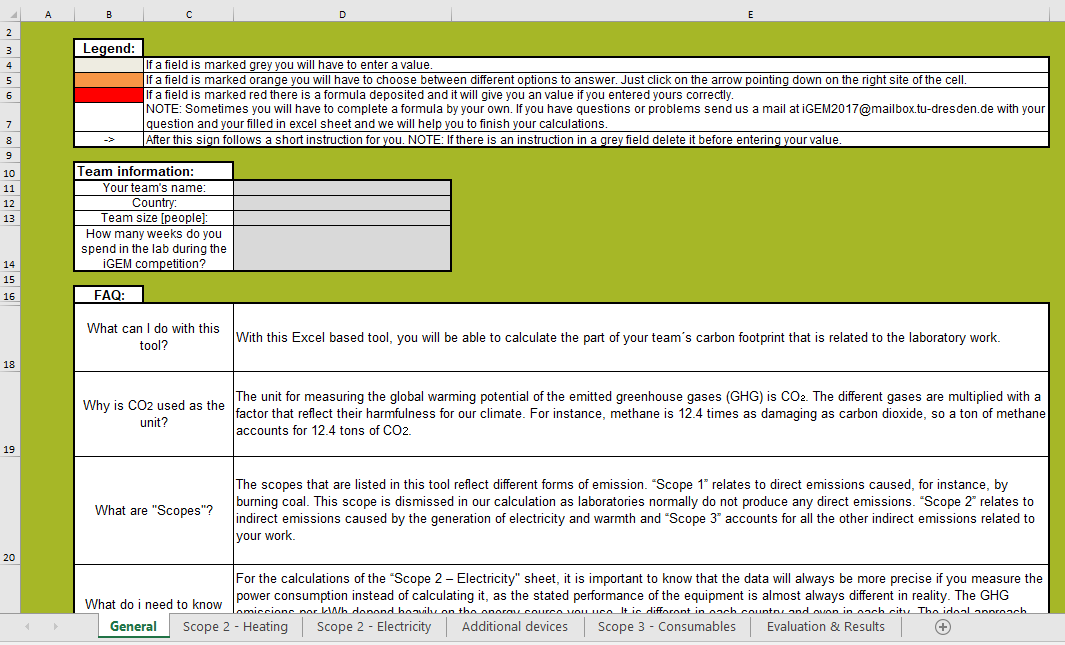
\includegraphics[width=\textwidth]{calculator_general.png}%
	\caption{General information}%
\end{figure}

\clearpage
\subsection{Scope 2}

Scope 2 – Heating implements that you heat your lab yourself or it is heated together with the rest of the building. If we want to be precise, air conditioning also belongs here. We haven’t been able to find any data about our lab. Instead, only annual consumption data for the whole building, also including office rooms etc., is recorded which is not suitable for our purposes.

\begin{figure}[h!]
	\centering
	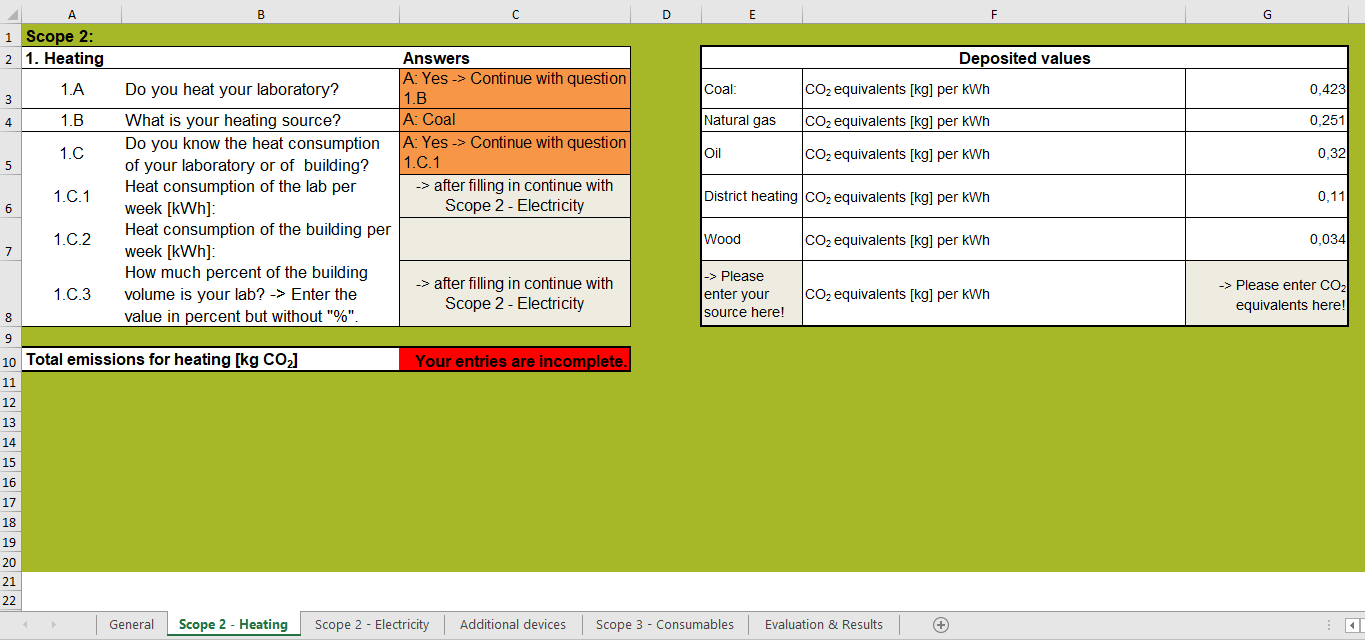
\includegraphics[width=\textwidth]{calculator_scope2a.png}%
	\caption{Do you have data about heating for your lab? If yes, include them in this sheet.}%
\end{figure}


For the calculations of the “Scope 2 – Electricity" sheet, it is important to know that the data will always be more precise if you measure the power consumption instead of calculating it, as the stated performance of the equipment is almost always different in reality. The GHG emissions per kWh depend heavily on the energy source you use. It is different in each country and even in each city. The ideal approach would be to identify the GHG emission for the power mix of your city or at least of your country. You can also use the stated data which refers to the average power mix of Germany.

\begin{figure}[h!]
	\centering
	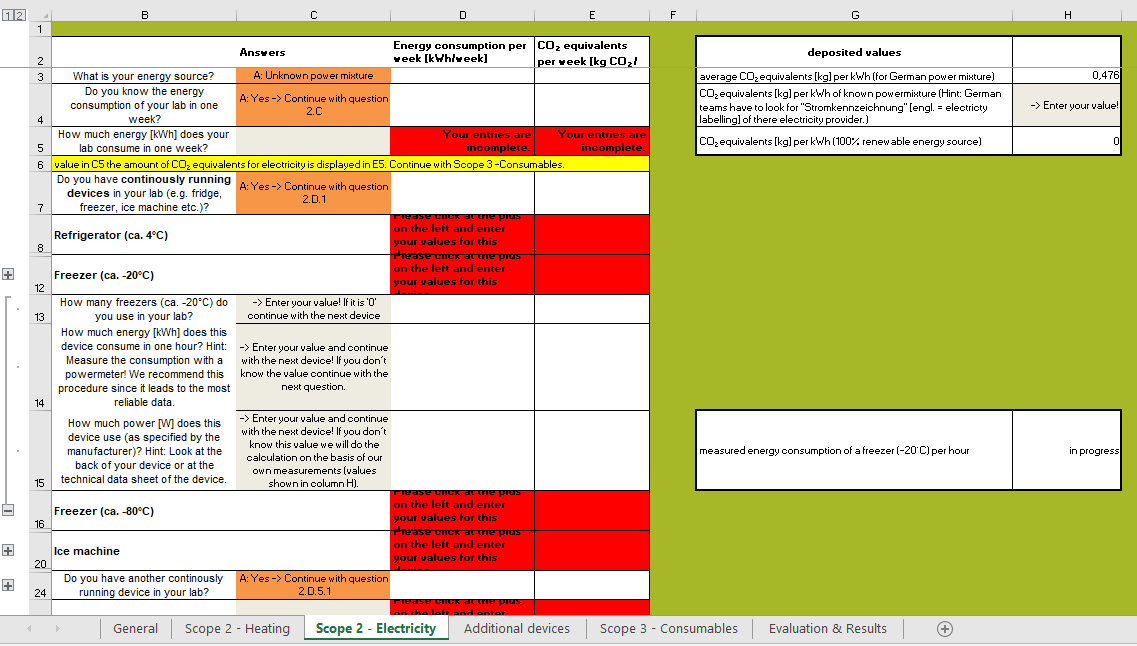
\includegraphics[width=\textwidth]{calculator_scope2b.png}%
	\caption{All electrical devices you use are listed here.}%
\end{figure}

In summary that means: try to get your hands on a powermeter and measure some runs of all your devices! If this is not possible, you don`t have any other option than calculating your energy consumption (usually gives higher values). 

\begin{suggest}{Track your device usage}
	To monitor how often and with which settings devices were used over a certain time (e.g. two weeks) we hang out lists and asked the users to fill them in whenever centrifuging, shaking etc. It worked out quite nicely!
\end{suggest}

If you have other devices we haven’t thought of yet, enter their values in the “Additional devices” sheet.
	
\begin{figure}[h!]
	\centering
	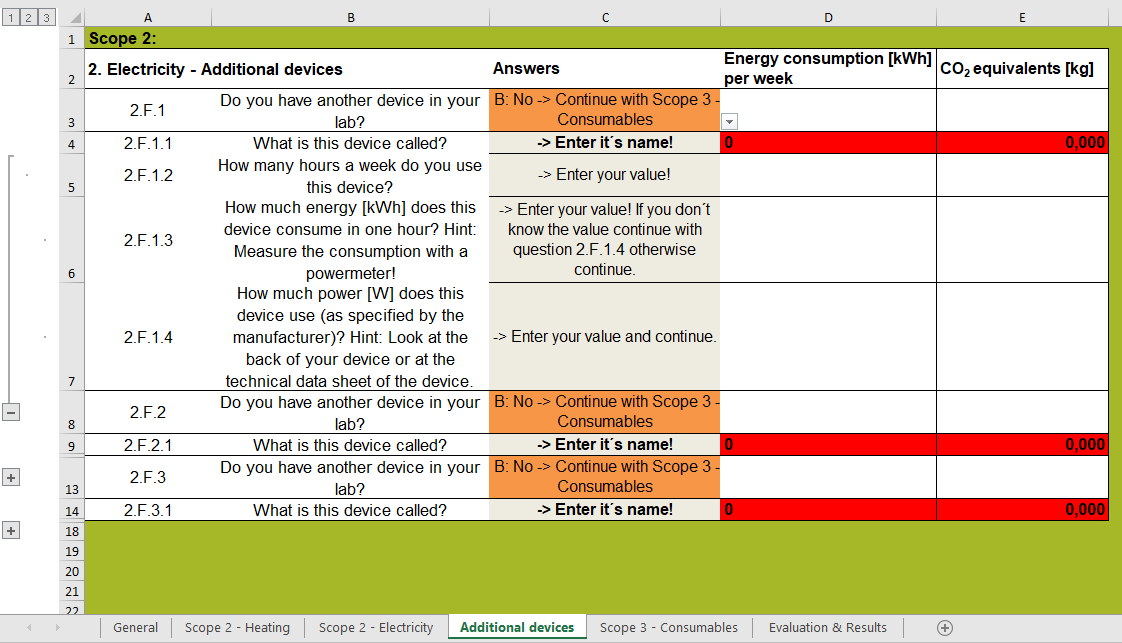
\includegraphics[width=\textwidth]{calculator_scope2c.png}%
	\caption{If you used additional devices we haven't thought of, enter their data here.}%
\end{figure}

\clearpage
\subsection{Scope 3}

"Scope 3" can include a lot of things. This could be the manufacturing of the products you use, the (environmental) cost of their shipping, your business trips, your daily commute and basically everything else you like to take in account. It is important to set the boundaries of your calculation at that point. Our team took in account the consumables and chemicals we use in our daily lab routine. They are interesting factors, as we hope to limit our consumption effectively after identifying the factors that add most to our footprint. The GHG emissions for “Scope 3” are normally measured from cradle to gate, meaning all of the production stages from the raw material up to the finished product leaving the gate of the factory are taken into account. We are not able to include the GHG emissions of the shipping, as these vary too much, but we would still like to encourage you to make collective orders to save on shipping. Neither included in our data are recycling or disposal of the used consumables and here again we would like to motivate you to separate your waste and recycle and reuse as much as possible. If you miss any items on the list of consumables, it is mostly due to the lack of data provided for that specific product. Especially the list of GHG emissions for chemicals is rather short. In many cases the data we do have is actually given for a similar or an intermediate product. Please treat the calculated results accordingly. The result will not reflect your real carbon footprint but it will give you an estimate. This estimate can be used to identify the prominent factors that add to your emissions and can give you an idea about the proportions of the impact the different factors have.

\begin{figure}[h!]
	\centering
	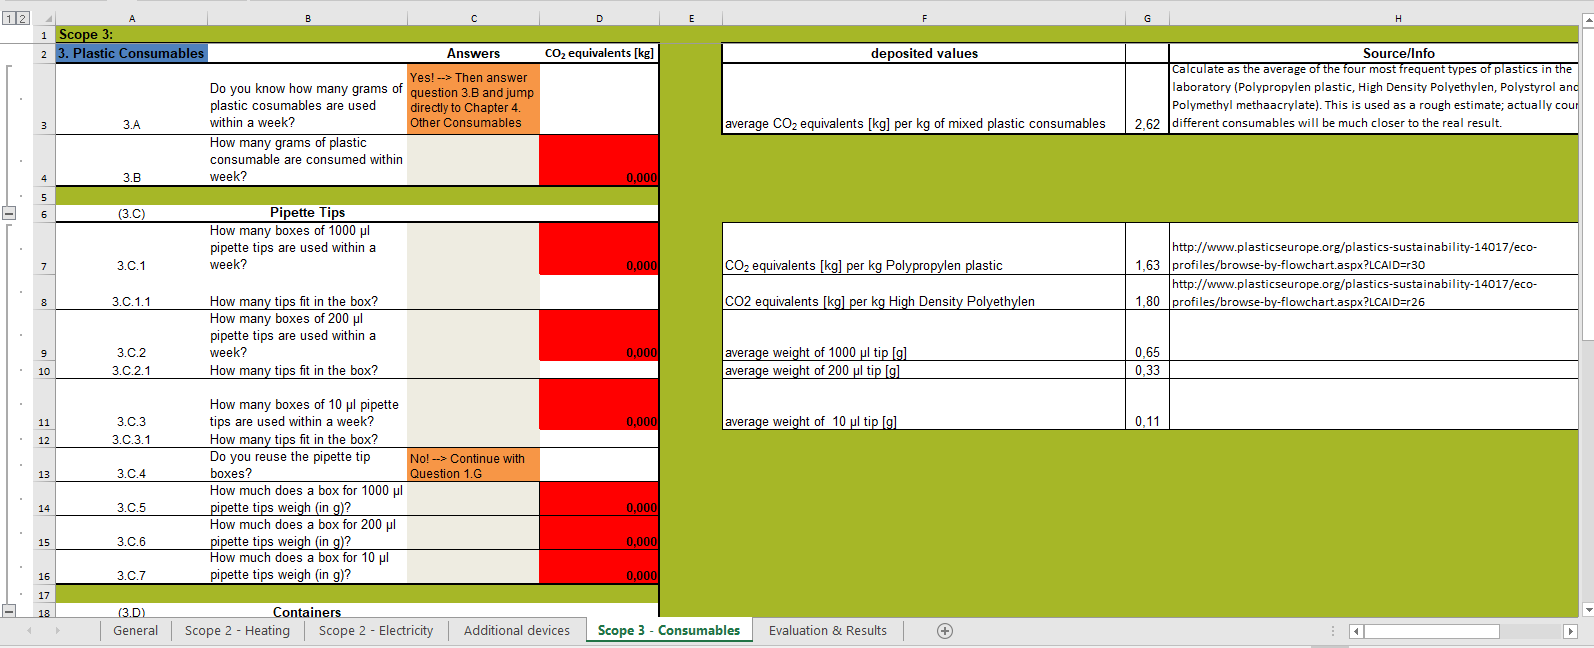
\includegraphics[width=\textwidth]{calculator_scope3.png}%
	\caption{Take into account the consumables and chemicals you use in your daily working routine in Scope 3.}%
\end{figure}

\begin{suggest}{Track your consumables}
	Make a tally to see how may pipette tip boxes, reaction tube packages, etc. are needed for a week in the lab. Alternatively, check your orders and see how much stuff is consumed over a (longer) time period.
\end{suggest}

\clearpage
\subsection{Evaluation and Results}

Have you entered all required data in the Exel sheet? Congratulations! Here’s the example of your calculation, we produced about 3520 kg CO$_2$ by our lab work.

\begin{figure}[h!]
	\centering
	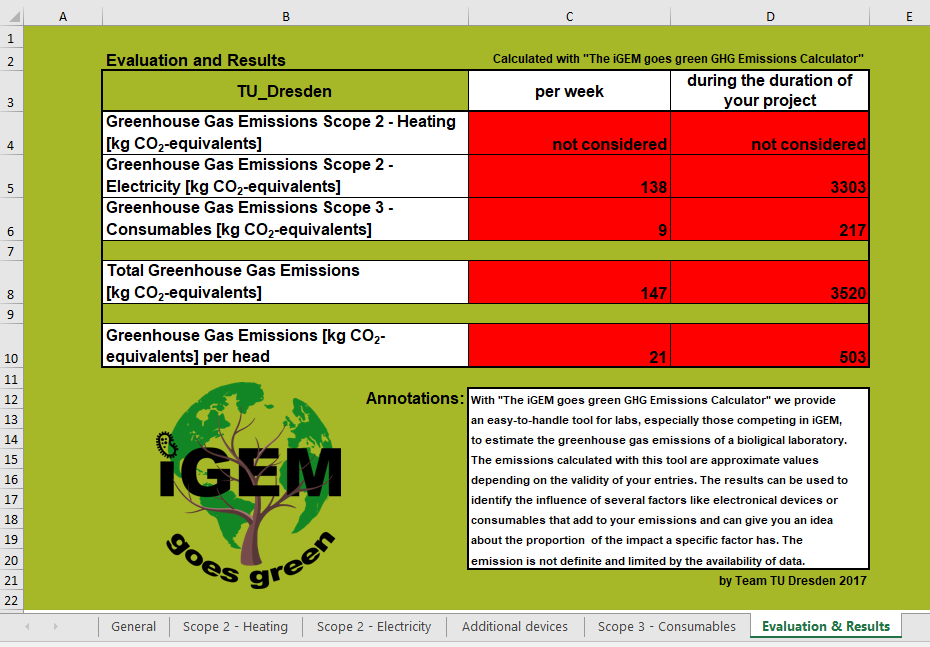
\includegraphics[width=\textwidth]{calculator_results.png}%
	\caption{Evaluation and Results of the emissions calculation of the TU Dresden 2017 iGEM team}%
\end{figure}

\begin{suggest}{Wanna help?}
	The data we will obtain with our measurements can be seen as a general estimation.
	However, the deviation between different devices and different producers might be huge. Consequently own measurements are advantageous for a precise calculation.\\
	We ask you to track your lab consumption of materials and energy. This will also help us to provide average numbers and gain a better estimation for teams all over the world. \\
	Interested? Just contact us and we will support you and your team!
	
\end{suggest}

\section{Meetups}

The emissions caused due to meetings and other events strongly rely on duration, number of participants and journey. \\
"Plant for the Planet" provides a useful online tool with the aim to have carbon neutral events. Therefore, the first step is the calculation of carbon emission, and that is exactly what we are looking for:

\begin{suggest} {Compensate your event} %TODO LINK 
	Plant for the planet offers an online tool to estimate how much carbon emissions are caused by your event. Go to \url{https://www.plant-for-the-planet.org/en/support/carbon-neutral-event} and have the following information ready:
	\begin{itemize}
		\item area of event location
		\item event duration
		\item number of participants
		\item transport (average distance, percentage of means of transport)
	\end{itemize}
\end{suggest}


\section{Flights and Travel}
Flights cause high emissions of greenhouse gases and therefore should be avoided whenever possible. Is there an alternative to get to the Giant Jamboree in Boston other then by plane (for those who don't live in North America)? By ship? *Joke* 


You see, flights usually can't be avoided. Nevertheless, nearly all means of transport (except for cycling and walking) cause emissions and in the end, all have to be taken into account. 
"Atmosfair", a German organization for climate protection, focuses on travel and provides a reliable online tool for travel emission calculations.


Below, we want to give a short list why we think the Atmosfair emission calculator is a trustful tool and why we highly recommend to apply it, especially for flights. 

\begin{itemize}
	\item A sufficient amount of independent data from scientific research projects was used to obtain numbers for nearly all combinations of factors. For example, if the user doesn't know the plane type, good estimations can be applied. Furthermore, factors with high impact on emissions are considered in detail, whereas factors with low impact are estimated.
	
	\item When burning kerosine, different pollutants having different effects are released (e.g. NO$_X$, CO$_2$ and particles). The resulting warming effect is calculated by transforming all effects into CO$_2$. Here, the "\textbf{R}adiative \textbf{F}orcing \textbf{I}ndex" (RFI) is used. It can only be applied in high altitudes above 9km and is not used for climbing up and landing phases. The calculator strictly separates between those phases.
	
	\item The methodology is validated by Germany's Federal Environmental Agency, promising highly reliable calculations.
\end{itemize}

The detailed description of methods and estimations used in this emission calculator can also be found on their website as pdf file (Documentation\_Calculator\_EN\_2008.pdf). \cite{flight_calc}%TODO: check out how that looks...

\begin{suggest} {Compensate your flights}
	Go to \url{https://www.atmosfair.de/en/home} and check out your travel emissions. If you want to use a different tool, please check where they got the data from, how it works in detail and which estimations are made. Don't use it before evaluating its trustworthiness!
\end{suggest}
